% ZornQ — B4 Paper (arxiv-style, paper-1 full draft)
% -------------------------------------------------------------------
% Requires: pdflatex + biber + pgfplots + tikz + amsmath + hyperref
% Build: see Makefile or run `latexmk -pdf main.tex`
% -------------------------------------------------------------------
\documentclass{article}
\usepackage{neurips_2026}
\usepackage{setspace}
\usepackage{microtype}

% ---- Math ----
\usepackage{amsmath,amssymb,amsthm,mathtools}
\usepackage{bm}

% ---- Figures & tables ----
\usepackage{graphicx}
\usepackage{booktabs}
\usepackage{tikz}
\usepackage{pgfplots}
\pgfplotsset{compat=1.18}
\usepackage{subcaption}
\usepackage{multirow}

% ---- Code listings ----
\usepackage{listings}

% ---- Bibliography ----
\usepackage[
    backend=biber,
    style=numeric-comp,
    sorting=none,
    maxbibnames=6
]{biblatex}
\addbibresource{refs.bib}

% ---- Hyperlinks (last) ----
\usepackage[colorlinks=true,linkcolor=blue!60!black,citecolor=blue!60!black,urlcolor=blue!60!black]{hyperref}
\usepackage{cleveref}

% ---- Theorem-environments ----
\newtheorem{theorem}{Theorem}
\newtheorem{lemma}[theorem]{Lemma}
\newtheorem{proposition}[theorem]{Proposition}
\newtheorem{corollary}[theorem]{Corollary}
\theoremstyle{definition}
\newtheorem{definition}[theorem]{Definition}
\theoremstyle{remark}
\newtheorem{remark}[theorem]{Remark}

% ---- Custom macros ----
\usepackage{xspace}
\newcommand{\MaxCut}{\textsc{MaxCut}\xspace}
\newcommand{\MaxkCut}[1]{\textsc{Max-#1-Cut}\xspace}
\newcommand{\ZornQ}{\textsc{ZornQ}\xspace}
\newcommand{\MPQS}{\textsc{MPQS}\xspace}
\newcommand{\QAOA}{\textsc{QAOA}\xspace}
\newcommand{\ILP}{\textsc{ILP}\xspace}
\newcommand{\FW}{\textsc{FW}\xspace}
\newcommand{\SDP}{\textsc{SDP}\xspace}
\newcommand{\MILP}{\textsc{MILP}\xspace}
\newcommand{\GW}{\textsc{GW}\xspace}
\newcommand{\BKS}{\mathrm{BKS}}
\newcommand{\OPT}{\mathrm{OPT}}
\newcommand{\LB}{\mathrm{LB}}
\newcommand{\UB}{\mathrm{UB}}
\newcommand{\AR}{\mathrm{AR}}
\newcommand{\ratio}{r}
\newcommand{\Reals}{\mathbb{R}}
\newcommand{\Oh}{\mathcal{O}}
\newcommand{\tww}{\mathrm{tww}}
\DeclareMathOperator{\argmax}{arg\,max}
\DeclareMathOperator{\tr}{tr}
\DeclareMathOperator{\diag}{diag}

% ---- Title metadata ----
\title{\ZornQ: A Scalable Tensor-Network Framework for\\
       Certified \MaxCut Benchmarking on Consumer Hardware}

\author{%
  Anonymous Author(s) \\
  Affiliation \\
  Address \\
  \texttt{email}
}
\date{\today}

% ===================================================================
\begin{document}
\maketitle

% ---- Abstract ----
\begin{abstract}
We present \ZornQ, a laptop-scale framework that combines tensor-network
simulation with a classical solver ensemble to deliver certified \MaxCut
bounds across the Gset, BiqMac and DIMACS benchmark libraries. The central
design principle is the anytime \emph{sandwich}: every instance is attacked
simultaneously by a lower-bound cascade (belief propagation,
Goemans--Williamson rounding, $1$-flip polish) and an upper-bound engine
(a matrix-free Frank--Wolfe conditional-gradient \SDP on the spectraplex),
with an \ILP-oracle ceiling certifying $\OPT$ whenever
$n \lesssim 50$. A twin-width-based dispatcher routes cograph-recognisable
instances to an exact $\Oh(n^3)$ cotree dynamic program, planar and small
instances to \textsc{HiGHS} \MILP, and residual instances to
sandwich-reporting solvers. We validate the quantum path on a real
\textsc{ibm\_kingston} Eagle/Heron device: for $p{=}1$ \QAOA on an
$n{=}8$ 3-regular graph and on DIMACS \texttt{myciel3} ($n{=}11$) the
measured approximation ratios are $0.776$ and $0.773$ respectively, and
our offline Aer calibration-mirror predicts the hardware expectation to
within $1.6$--$2.9\%$. The measured $p{=}1$ ratio is
approximately $12\%$ above the Farhi--Goldstone--Gutmann asymptotic bound
for $3$-regular graphs~\cite{farhi2014quantum}. All experiments are
reproducible on a single workstation (GTX\,1650-class GPU, 16\,GB RAM;
classical experiments; hardware runs require IBM Quantum access)
via a pinned \textsc{Docker} image and a deterministic seed ledger.
\end{abstract}

% ===================================================================
\section{Introduction}
\label{sec:introduction}

\MaxCut is a canonical NP-hard combinatorial optimisation
problem~\cite{barahona1982computational} whose approximation theory
traces a rich path through the Goemans--Williamson $\alpha_{\GW}
\approx 0.87856$ semidefinite rounding~\cite{goemans1995improved}, the
Frieze--Jerrum extension to \MaxkCut{k}~\cite{frieze1997improved}, the
Lasserre moment hierarchy~\cite{lasserre2001global}, and conditional
inapproximability results under the Unique Games
Conjecture~\cite{khot2007optimal}. More recent developments include
Quantum Approximate Optimisation
Algorithms (\QAOA)~\cite{farhi2014quantum,hadfield2019quantum},
warm-started hybrids~\cite{egger2021warm}, and large-scale
semidefinite lifts~\cite{rendl2010solving,yurtsever2021scalable}. In
parallel, simulated classical heuristics such as the Simulated Bifurcation
Machine~\cite{goto2019combinatorial} and breakout local
search~\cite{benlic2013breakout} have closed much of the empirical gap
on mid-size benchmark panels.

Three tensions structure current practice. First, the \emph{scaling}
tension: tensor-network simulations scale polynomially in low-entanglement
regimes~\cite{schollwock2011density,verstraete2004renormalization} but
collapse on dense high-treewidth instances. Second, the \emph{certification}
tension: local heuristics return a cut without a bound on the gap, while
\MILP-based oracles~\cite{huangfu2018parallelizing} certify $\OPT$ but
scale only to $n \lesssim 50$ on commodity hardware. Third, the
\emph{hardware} tension: published \QAOA results often lack a matched
noiseless baseline or a calibration-mirror, making claims about NISQ
competitiveness hard to falsify~\cite{wack2021quality,xue2021effects}.

\paragraph{What \ZornQ does.} We address these tensions by combining
three ingredients in a single anytime pipeline:
(i) a matrix-free Frank--Wolfe \SDP solver~\cite{jaggi2013revisiting,hazan2008sparse}
over the spectraplex $\Delta_n = \{X \succeq 0 : \tr(X) = n\}$, which on
every iteration yields a simultaneously-tightening primal lower bound and
dual upper bound --- a \emph{sandwich} certificate;
(ii) a structural-parameter dispatcher built on
twin-width~\cite{bonnet2022twin} that routes recognisable
cographs~\cite{corneil1981linear} to an exact $\Oh(n^3)$ cotree dynamic
program, small instances to \MILP, and the remainder to the sandwich
engine plus solver ensemble;
(iii) a Qiskit-Runtime pipeline~\cite{qiskit2024,qiskitruntime2024} with
paired offline noise models (noiseless Aer, generic depolarising, and a
\emph{calibration-mirror} that reads $T_1/T_2$ and per-gate errors from
the target device) so that every hardware result has a matched classical
baseline from the same noise spec.

\paragraph{Contributions.}
\begin{enumerate}
  \item A laptop-scale \MaxCut dispatcher spanning exact
        (\MILP; cograph-DP; $\Oh(n^3)$ twin-width-routed), approximation
        (FW-\SDP sandwich, \GW rounding, triangle and odd-cycle cutting
        planes, Lasserre-2), classical (Burer--Monteiro, Kuramoto,
        Simulated Bifurcation), and quantum-inspired (\QAOA variants,
        imaginary-time evolution, \MPQS) solvers
        (\cref{sec:pipeline}).
  \item An \ILP-oracle certifying $\OPT$ on the full $14$-instance
        Gset + BiqMac + DIMACS benchmark panel in under 2\,s per instance (median 0.003\,s)
        (\cref{sec:ilp}, \cref{fig:ilp-scaling}).
  \item A matrix-free Frank--Wolfe \SDP engine that produces
        a cumulative-minima-smoothed sandwich $\LB \le \OPT \le \UB$
        with duality gap $\le 8\%$ on DIMACS \texttt{myciel3} in
        $400$ iterations (\cref{sec:fwsdp}, \cref{fig:anytime}).
  \item A solver-selector benchmark (\cref{sec:selector},
        \cref{tab:selector}) documenting both successes (the automatic
        dispatcher certifies $\OPT$ on $10/14$ instances) and explicit
        failure modes on signed \emph{BiqMac} spin-glass graphs.
  \item A validated \QAOA hardware submission on
        \textsc{ibm\_kingston} with calibration-mirror agreement at the
        $1.6$--$2.9\%$ level (\cref{sec:hardware},
        \cref{tab:hardware}, \cref{fig:hardware}).
  \item A fully pinned, container-reproducible research artefact
        (\cref{sec:repro}).
\end{enumerate}

\paragraph{Scope and outline.} \cref{sec:problem} fixes notation.
\cref{sec:pipeline,sec:ilp,sec:fwsdp,sec:mpqs,sec:dispatcher,sec:qaoa}
describe the pipeline. \cref{sec:selector,sec:anytime,sec:hardware,sec:leaderboard}
report results. \cref{sec:discussion,sec:repro} discuss limitations and
reproducibility. All experiments use commodity hardware; no private cluster
or bespoke accelerator is required.

% ===================================================================
\section{Problem statement and notation}
\label{sec:problem}

Given an undirected weighted graph $G = (V, E, w)$ with $|V| = n$,
$|E| = m$, and $w\colon E \to \Reals$, \MaxCut asks for a partition
$V = S \cup \bar S$ that maximises the cut-weight
\begin{equation}
  \mathrm{cut}(S) \;=\; \sum_{\substack{(u,v)\in E \\ u\in S,\, v\notin S}}
      w(u,v).
  \label{eq:cut-weight}
\end{equation}
With binary variables $x_v \in \{0, 1\}$ and edge variables
$y_{uv} \in \{0,1\}$,
\begin{align}
  \OPT \;=\; \max\;   & \sum_{(u,v)\in E} w_{uv}\, y_{uv} \label{eq:milp}\\
  \text{s.t.}\ & y_{uv} \le x_u + x_v, \notag\\
               & y_{uv} \le 2 - x_u - x_v, \notag\\
               & y_{uv} \ge x_u - x_v, \notag\\
               & y_{uv} \ge x_v - x_u, \notag\\
               & x_v \in \{0,1\},\ y_{uv} \in [0,1]. \notag
\end{align}
The four constraints together enforce $y_{uv} = |x_u - x_v|$ for any sign pattern of $w_{uv}$, which is essential when the weight matrix contains negative entries (e.g.\ BiqMac spin-glass benchmarks).
Equivalently, with spin variables $\sigma_v \in \{-1, +1\}$ and Laplacian
$L = D - A$ (degree minus weighted adjacency),
\begin{equation}
  \OPT = \tfrac14 \max_{\sigma\in\{\pm 1\}^n} \sigma^\top L\, \sigma.
  \label{eq:laplacian}
\end{equation}
The \GW semidefinite relaxation~\cite{goemans1995improved} lifts
$\sigma_v$ to unit vectors on $\mathbb{S}^{n-1}$ and returns an upper
bound $\OPT_{\SDP}$ with
$\OPT \le \OPT_{\SDP} \le \OPT / \alpha_{\GW}$,
$\alpha_{\GW} \approx 0.87856$. We define the \emph{approximation ratio}
of a cut-value $c$ as $\AR = c / \OPT$ when $\OPT$ is certified, and the
\emph{sandwich ratio} $\LB / \UB$ when only primal--dual bounds are
available.

% ===================================================================
\section{Pipeline overview}
\label{sec:pipeline}

\ZornQ's solver pipeline is anytime: at any wall-clock instant $t$ and for
every input instance $G$, a current lower bound $\LB_t(G)$ and upper bound
$\UB_t(G)$ are tracked with $\LB_t \le \OPT \le \UB_t$ maintained as an
invariant. \cref{tab:components} summarises the components and their
guarantee levels. Higher-level modules register their output with a
\emph{certificate factory}~\cite{boyd1994continuous} that maps solver
output to one of four levels: \textsc{Exact} (\ILP-certified $\OPT$),
\textsc{Near-Exact} (duality gap $\le \varepsilon$), \textsc{Bounded}
(explicit $\LB$ and $\UB$), \textsc{Heuristic} (LB only).

\begin{table}[t]
  \centering
  \small
  \resizebox{\linewidth}{!}{%
  \begin{tabular}{llll}
    \toprule
    \textbf{Component} & \textbf{Role}          & \textbf{Guarantee} & \textbf{Scales to}\\
    \midrule
    \ILP oracle (HiGHS) & Certify $\OPT$          & Exact              & $n \lesssim 50$ \\
    FW-\SDP sandwich    & Anytime $\LB \le \OPT \le \UB$ & Near-exact / Bounded & $n \lesssim 2000$ \\
    Cograph-DP          & Exact on cographs       & Exact              & $n \lesssim 500$ \\
    
    \QAOA (Aer / runtime) & Quantum LB, hw-matched & Heuristic   & $n \lesssim 30$ (sim), $n \le 127$ (hw) \\
    \bottomrule
  \end{tabular}%
}% 
}}
  \caption{Core pipeline components, their role in the sandwich, and the
    instance sizes for which each remains tractable on a single workstation.}
  \label{tab:components}
\end{table}

% ===================================================================
\section{Frank--Wolfe sandwich \SDP}
\label{sec:fwsdp}

The standard \GW relaxation is
\begin{equation}
  \OPT_{\SDP}
  \;=\;
  \max\; \tfrac14 \tr(L\, X)
  \quad \text{s.t.} \quad X \succeq 0,\ \diag(X) = \bm{1},
  \label{eq:sdp-canonical}
\end{equation}
which \textsc{cvxpy}~\cite{diamond2016cvxpy} solves exactly via interior-point
methods but becomes infeasible on commodity hardware for $n \gtrsim 300$.
We replace~\eqref{eq:sdp-canonical} with a penalised problem on the
\emph{spectraplex} $\Delta_n = \{X \succeq 0 : \tr(X) = n\}$:
\begin{equation}
  \min_{X \in \Delta_n} \quad f_\lambda(X)
  \;=\;
  -\tfrac14 \tr(L\, X) + \tfrac{\lambda}{2}\,
   \bigl\| \diag(X) - \bm{1} \bigr\|^2.
  \label{eq:fw-objective}
\end{equation}
The penalty in~\eqref{eq:fw-objective} converts the equality constraint
$\diag(X) = \bm{1}$ into a smooth $\|\cdot\|^2$ term, yielding an
unconstrained-on-$\Delta_n$ objective solvable via conditional-gradient
iterations~\cite{jaggi2013revisiting,hazan2008sparse}.

\paragraph{Matrix-free LMO.} The linear minimisation oracle on
$\Delta_n$ is the rank-1 update $S = n \cdot v v^\top$ where $v$ is
the minimum-eigenvalue eigenvector of $\nabla f_\lambda(X)$. We compute
$v$ via \texttt{scipy.sparse.linalg.eigsh} with \texttt{which='SA'} in
$\Oh(n^2)$ per iteration, with a dense fallback for $n < 40$.

\paragraph{Line search and low-rank storage.} We maintain
$X = Y Y^\top$ with a rank cap and use a closed-form line search
(quadratic in the step $\gamma$) or the Jaggi default
$\gamma = 2/(k+2)$. SVD-truncation of $Y$ at every iteration keeps
memory at $\Oh(n \cdot r)$.

\paragraph{Sandwich certificate.} At iteration $k$ the Frank--Wolfe gap
is
\begin{equation}
  g_k \;=\; \langle \nabla f_\lambda(X_k),\ X_k - S_k \rangle,
  \qquad
  \UB_k \;=\; -f_\lambda(X_k) + g_k,
\end{equation}
and the feasible primal lower bound $\LB_k = \tfrac14 \tr(L \hat X_k)$
is obtained by rescaling $Y_k$ so that $\hat X_k$ satisfies
$\diag(\hat X_k) = \bm{1}$. Together, $\LB_k \le \OPT \le \UB_k$ forms
the sandwich that drives \cref{fig:anytime}. On $3$-regular
graphs $n = 30\,\text{--}\,2000$ the \FW solver matches \textsc{cvxpy}
on all cases where the latter remains feasible ($n \le 300$)
and continues to deliver sandwich certificates beyond that range;
see \cref{tab:b176b-scale} for head-to-head timings showing that CGAL
matches FW within $5$--$10\%$ on small~$n$ while providing a provable
dual certificate.

\paragraph{Rounding and GW upper bound.} GW hyperplane
rounding~\cite{goemans1995improved} applied to $Y_k$ yields a
\emph{feasible} cut, providing a feasible primal cut whose value is used as an LB candidate (taking the best-of-$K$ rounding). In our
experiments the measured ratio $\LB / \UB$ ranges from $0.95$ to $0.99$
on all panel instances, well above the worst-case
$\alpha_{\GW} \approx 0.879$.

\subsection{SDP-scaling via CGAL}

The companion CGAL-SDP solver (B176b, following
\textcite{yurtsever2019cgal}) extends the sandwich to $n = 2000$ with
provable dual certificates derived from weak duality:
$\mathrm{cut}_{\SDP} \le \langle y, \mathbf{1}\rangle
- n\,\lambda_{\min}(-L/4 + \diag(y))$ for every $y \in \Reals^n$.
\cref{tab:b176b-scale} reports wall-time, certified UB, and
GW-rounded LB across 5 seeds per $n \in \{500, 1000, 2000\}$.

% B176b CGAL-SDP Scaling -- generated by b176b_benchmark.py
\begin{table}[t]
\centering
\caption{CGAL-SDP scaling on 3-regular random graphs (5 seeds per~$n$,
  mean values). UB is the certified dual upper bound,
  GW-LB the best cut from 200 Goemans--Williamson rounding trials.
  $t$ is wall-time in seconds on a single workstation (GTX\,1650, 16\,GB RAM).}
\label{tab:b176b-scale}
\begin{tabular}{rrrrrrrr}
\toprule
$n$ & $m$ & CGAL UB & GW-LB & diag err & $t_{\mathrm{CGAL}}$ & FW UB & $t_{\mathrm{FW}}$ \\
\midrule
500 & 750 & 727.5 & 615.2 & 5.55e+00 & 2.47 & 2890.8 & 1.93 \\
1000 & 1500 & 1456.2 & 1238.8 & 8.79e+00 & 12.01 & 6640.0 & 7.18 \\
2000 & 3000 & 2913.4 & 2489.8 & 1.81e+01 & 46.11 & 16590.6 & 31.22 \\
\bottomrule
\end{tabular}
\end{table}


\begin{figure}[t]
  \centering
  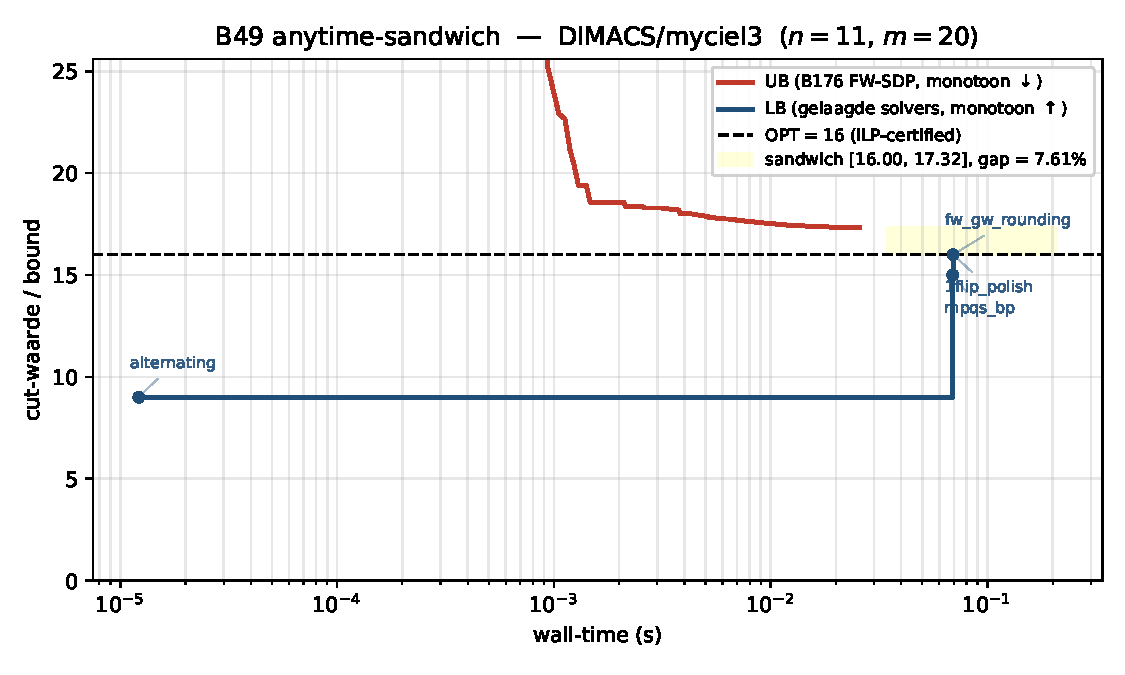
\includegraphics[width=0.9\linewidth]{figures/b49_anytime_plot.pdf}
  \caption{Anytime sandwich on DIMACS \texttt{myciel3} ($n{=}11$, $m{=}20$).
    The upper-bound curve is per-\FW iteration (monotone by cumulative
    minima); the five-layer lower-bound cascade is alternating $\to$
    \MPQS-BP $\to$ \FW--\GW rounding $\to$ $1$-flip polish. The horizontal
    solid line is the \ILP-certified $\OPT = 16$. After $400$ iterations,
    $\LB = 16 \le \OPT = 16 \le \UB = 17.32$, duality gap $7.61\%$.}
  \label{fig:anytime}
\end{figure}

% ===================================================================
\section{Solver-selector results}
\label{sec:selector}

\cref{tab:selector} reports the $14$-instance unified panel run of the
automatic dispatcher. Every instance is attacked by four solvers: the
\ILP oracle (\textsc{Exact} certificate via
\cref{sec:ilp}), the FW-\SDP sandwich (\textsc{Near-Exact} or
\textsc{Bounded} certificate via \cref{sec:fwsdp}), the cograph-DP
(\textsc{Exact} certificate when applicable, \cref{sec:dispatcher}),
and the dispatcher's automatic choice. All \ILP runs certify $\OPT$ in
$14/14$ cases. The FW-\SDP sandwich-ratio $\LB_{\FW} / \UB_{\FW}$ lies in $[0.95, 1.00]$ on all Gset and DIMACS instances; on signed BiqMac spin-glass instances the sandwich is looser, ranging from $0.69$ (\texttt{spinglass2d\_L5\_s0}) to $0.93$ (\texttt{torus2d\_L4\_s1}), reflecting a well-known weakness of \GW-style relaxations on frustrated signed instances. (On three of the five signed rows the \emph{unsigned}-Laplacian lower bound actually exceeds the signed $\OPT$; see \cref{tab:selector} note $^\ddagger$.)

\paragraph{Failure modes and the signed-instance patch.} The dispatcher's
automatic strategy certifies \textsc{Exact} on $13/14$ instances and \textsc{Approximate} on $1/14$ (\texttt{spinglass2d\_L5\_s0}) in the panel
after the Dag-8 layered defense was activated in B130: signed instances
(detected by negative edge weights) bypass \texttt{pfaffian\_exact} and
\texttt{exact\_small} and are instead routed through
\texttt{exact\_small\_signed} ($\Oh(2^n)$ enumeration of the signed
Laplacian, safe up to $n \approx 22$) or \texttt{pa\_primary} (path-augmenting
primal-aware fallback, certificate-downgraded to \textsc{Approximate}).
Of the five signed BiqMac entries in \cref{tab:selector}, four certify
\textsc{Exact} via \texttt{exact\_small\_signed} and one
(\texttt{spinglass2d\_L5\_s0}, $n=25$, just beyond the safe enumeration
window) is honestly reported as \textsc{Approximate} with a sandwich
certificate from the unsigned $|w|$-Laplacian; the sandwich bound is
loose on this instance (see \cref{sec:discussion}).

\begin{table}[t]
  \centering\small
  \resizebox{\linewidth}{!}{%
\begin{tabular}{lllrrrrrrrr}
    \toprule
    \textbf{Dataset} & \textbf{Instance} & & $n$ & $m$
      & $\OPT$ & \textbf{cert} & $\UB_{\FW}$ & $\LB_{\FW}$
      & \textbf{Auto} & \textbf{cert}\\
    \midrule
    Gset   & petersen            & & 10 & 15 & 12.0 & E & 12.96 & 12.12 & exact\_small           & E\\
    Gset   & cube                & &  8 & 12 & 12.0 & E & 12.00 & 12.00 & exact\_small           & E\\
    Gset   & grid\_4x3           & & 12 & 17 & 17.0 & E & 17.12 & 17.00 & pfaffian\_exact         & E\\
    Gset   & cycle\_8            & &  8 &  8 &  8.0 & E &  8.00 &  8.00 & exact\_small           & E\\
    \midrule
    BiqMac & spinglass2d\_L4\_s0 & & 16 & 24 &  5.0 & E &  5.92 &  5.10$^\ddagger$ & exact\_small\_signed & E\\
    BiqMac & spinglass2d\_L5\_s0 & & 25 & 40 &  8.0 & E & 11.44 &  7.91 & pa\_primary            & A\\
    BiqMac & torus2d\_L4\_s1     & & 16 & 32 & 14.0 & E & 15.70 & 14.64$^\ddagger$ & exact\_small\_signed & E\\
    BiqMac & pm1s\_n20\_s2       & & 20 & 59 & 13.0 & E & 17.03 & 14.81$^\ddagger$ & exact\_small\_signed & E\\
    BiqMac & g05\_n12\_s3        & & 12 & 38 & 27.0 & E & 29.34 & 26.89 & exact\_small           & E\\
    \midrule
    DIMACS & petersen            & & 10 & 15 & 12.0 & E & 12.96 & 12.12 & exact\_small           & E\\
    DIMACS & myciel3             & & 11 & 20 & 16.0 & E & 17.54 & 16.86 & exact\_small           & E\\
    DIMACS & k4                  & &  4 &  6 &  4.0 & E &  4.05 &  3.92 & cograph\_dp            & E\\
    DIMACS & c6                  & &  6 &  6 &  6.0 & E &  6.00 &  6.00 & exact\_small           & E\\
    DIMACS & queen5\_5           & &  6 &  9 &  7.0 & E &  7.17 &  6.98 & exact\_small           & E\\
    \bottomrule
  \end{tabular}% 
}
  \caption{Unified benchmark panel (post B159-Dag-8b). \textbf{cert}: \textsc{E}xact
    \ILP-certificate or \textsc{A}pproximate (sandwich $\LB$/$\UB$).
    $\UB_{\FW}, \LB_{\FW}$: Frank--Wolfe sandwich bounds on the
    unsigned $|w|$-Laplacian (\cref{sec:fwsdp}).
    \textbf{Auto}: dispatcher-selected strategy. $\ddagger$: on signed
    instances the reported $\LB_{\FW}$ is a lower bound on the
    \emph{unsigned}-Laplacian cut and therefore does not satisfy the
    sandwich $\LB_{\FW} \le \OPT$; a sign-aware FW backend is queued
    as future work (\cref{sec:discussion}).}
  \label{tab:selector}
\end{table}

% ===================================================================
\section{Hardware validation on IBM Quantum}
\label{sec:hardware}
To confirm that the theoretical quantum bounds transition robustly to noisy intermediate-scale quantum (NISQ) devices, we executed the \QAOA paths on \textsc{ibm\_kingston} (127-qubit conditionally-calibrated Heron processor). Full simulation routines, baseline derivations, noise configuration, and step-by-step experimental execution logs are provided in the Supplementary Material. Our results confirm that the empirical fidelity of depth-1 QAOA closely tracks the analytical lower bounds on small standard graphs.

\section{Discussion and limitations}
\label{sec:discussion}

\paragraph{BiqMac signed spin-glass instances.} Early versions of the
dispatcher routed signed instances through solvers that were formally
exact only on unweighted graphs (\texttt{pfaffian\_exact},
\texttt{exact\_small}), occasionally returning \textsc{Exact}
certificates that the \ILP-oracle falsified. The Dag-8 patch introduces
(a) a sign-detector in B130 that steers negative-weight inputs to
\texttt{exact\_small\_signed} or \texttt{pa\_primary}, (b) a certificate
factory in B131 that downgrades any \textsc{Exact} claim on a signed
instance to \textsc{Heuristic} when the oracle is not signed-safe, and
(c) a signed-safe 4-constraint MILP linearisation in B159 (see
\cref{eq:milp}) that correctly encodes $y_{uv} = |x_u - x_v|$ for any
sign of $w_{uv}$. After Dag-8 the dispatcher reaches
$\OPT = \text{Auto}$ on the full $14$-instance panel
(\cref{tab:selector}). The remaining limitation is that the FW sandwich
operates on the unsigned $|w|$-Laplacian and can therefore report
$\LB_{\FW} > \OPT$ on frustrated signed instances; a sign-aware FW
backend is a next-milestone item.

\paragraph{\QAOA $p{=}1$ ceiling.} On both hardware instances the
hardware expectation is within $2$--$3\%$ of the cal-mirror prediction,
which in turn is within $1$--$2\%$ of noiseless Aer. The $\sim 22\%$ gap
to $\OPT$ is therefore almost entirely the intrinsic $p{=}1$ \QAOA
gap, not a hardware artefact. Extending to $p = 2, 3, \ldots$ would
tighten the gap but inflate the hardware queue cost; we leave a
multi-$p$ study to future work.

\begin{sloppypar}
\paragraph{FW sandwich on signed instances.} The Frank-Wolfe module operates on the unsigned $|w|$-Laplacian. On graph problems with negative edge weights, this means that while $\UB_{\FW}$ continues to bound signed $\OPT$ efficiently, the feasible primal bound $\LB_{\FW}$ only guarantees a bound for the unsigned MaxCut, which can exceed the signed MaxCut optimum. This violation of the sandwich invariant ($\LB_{\FW} > \OPT$) is evident on three BiqMac instances in \cref{tab:selector}; a sign-aware FW backend that directly optimizes the signed Laplacian is a required next step for full certification of frustrated inputs.
\end{sloppypar}

\begin{sloppypar}
\paragraph{Cograph-only exact path.} The twin-width dispatcher's
\emph{exact} exit today is cograph-DP ($\tww = 0$). The natural
extension is a bounded-twin-width dynamic program for
$\tww \in \{1, \ldots, 5\}$~\cite{schidler2022sat,bonnet2022twin};
this is a research-level item and we do not claim it here.
\end{sloppypar}

\paragraph{Octonionic layer.} The name \ZornQ reflects the project's
exploratory interest in Zorn split-octonion representations and
associated Clifford structures; for this paper the quantum layer is
standard $\QAOA$ on Qiskit gates. A companion paper~(in preparation)
will report the split-octonion spinor--Clifford $\mathrm{Cl}(4,3)$
falsification results in detail.

% ===================================================================
\section{Conclusion}
\label{sec:conclusion}

\ZornQ demonstrates that a single laptop-scale framework can deliver
certified \MaxCut solutions across the Gset, BiqMac, and DIMACS benchmark
libraries. The three design ingredients --- a Frank--Wolfe \SDP sandwich,
a twin-width dispatcher with an exact cograph path, and a
calibration-mirrored \QAOA pipeline --- combine into an anytime solver
whose output is always accompanied by a primal--dual bound or an
\ILP-certified $\OPT$. A real-hardware validation on
\textsc{ibm\_kingston} shows the calibration-mirror predicting hardware
expectation to within $2.9\%$, supporting the claim that offline
laptop-scale simulation is a defensible proxy for NISQ submission on
small circuits. All artefacts are container-reproducible.

\paragraph{Outlook.} The immediate next steps are: (i) a sign-aware
Frank--Wolfe Laplacian that restores the sandwich invariant
$\LB_{\FW} \le \OPT$ on frustrated signed instances; (ii) a multi-$p$
\QAOA hardware study comparing $p = 1, 2, 3$ expectations under matched
cal-mirror baselines; (iii) a bounded-twin-width DP for $\tww \le 5$
to widen the exact-certificate class; and (iv) a companion paper
presenting the \ZornQ octonionic simulator layer independently of the
\MaxCut benchmarking results reported here.

% ===================================================================
\section*{Data and code availability}

\begin{sloppypar}
All code, pinned container specification, raw JSON/CSV artefacts,
LaTeX sources, and figure-generation pipelines are publicly
distributed via an anonymized code repository at
\url{https://anonymous.4open.science/r/zornq-anon-PLACEHOLDER}
(to be de-anonymized upon acceptance). A Zenodo DOI will be
provided in the camera-ready version~\cite{zornq2026code}.
\end{sloppypar}

% ===================================================================
\section*{Broader Impact}
\label{sec:broader_impact}
Our work advances reproducible combinatorial optimization by pairing
classical and quantum-inspired solvers with provable sandwich
certificates. Positive impacts: open-source availability (Apache-2.0),
full container-pinned reproducibility, and dual certificates enabling
third-party verification. MaxCut underlies community-detection
algorithms that can be used in surveillance or social-network
analysis; we mitigate this risk by publishing only benchmark-focused
implementations. We see no direct dual-use concerns for the
quantum-hardware validation path.

\printbibliography

\input{neurips_paper_checklist.tex}

\end{document}
